\experiment{Queue Using Linked List}{14/11/2023}

\section{Aim}
Write a menu driven C Program to implement a queue using linked list with the following
operations:
\\a. Insert elements to the queue.
\\b. Delete elements from the queue.
\\c. Display the queue after each operation

\section{Algorithm}
 {\fontfamily{lmtt}\selectfont

  \subsection{Structure Definition}
  Create a structure \texttt{Node} with the following attributes:
  \begin{enumerate}[label=\arabic*:,left=0pt]
    \item Integer \texttt{data} to store the data of the node.
    \item Pointer to \texttt{Node} \texttt{next} to store the address of the next node.
  \end{enumerate}

  \subsection{Display Function}
  Create a function \texttt{display(head)}:
  \begin{enumerate}[label=\arabic*:,left=0pt]
    \item \textbf{Start}
    \item If \texttt{head} is \texttt{NULL}, print "The Queue is empty!" and return.
    \item Print a newline.
    \item Create a \texttt{Node} pointer \texttt{current} and set it to \texttt{head}.
    \item Loop while \texttt{current} is not \texttt{NULL}:
          \begin{enumerate}[label=2.\arabic*:, start=1]
            \item Print \texttt{current->data} followed by a space.
            \item Set \texttt{current} to \texttt{current->next}.
          \end{enumerate}
    \item Print a newline.
    \item \textbf{Stop}
  \end{enumerate}

  \subsection{InsertBegin Function}
  Create a function \texttt{insertBegin(head, data)}:
  \begin{enumerate}[label=\arabic*:,left=0pt]
    \item \textbf{Start}
    \item Allocate memory for a new \texttt{Node} structure using \texttt{malloc}.
    \item Set \texttt{temp->next} to \texttt{head}.
    \item Set \texttt{temp->data} to \texttt{data}.
    \item Set \texttt{head} to \texttt{temp}.
    \item Return \texttt{head}.
    \item \textbf{Stop}
  \end{enumerate}

  \subsection{DeleteEnd Function}
  Create a function \texttt{deleteEnd(head)}:
  \begin{enumerate}[label=\arabic*:,left=0pt]
    \item \textbf{Start}
    \item If \texttt{head} is \texttt{NULL}, print "List is empty!" and return \texttt{head}.
    \item If \texttt{head->next} is \texttt{NULL}:
          \begin{enumerate}[label=3.\arabic*:, start=1]
            \item Free \texttt{head}.
            \item Set \texttt{head} to \texttt{NULL}.
            \item Return \texttt{head}.
          \end{enumerate}
    \item Create a \texttt{Node} pointer \texttt{current} and set it to \texttt{head}.
    \item Create a \texttt{Node} pointer \texttt{prev}.
    \item Loop while \texttt{current->next} is not \texttt{NULL}:
          \begin{enumerate}[label=3.\arabic*:, start=1]
            \item Set \texttt{prev} to \texttt{current}.
            \item Set \texttt{current} to \texttt{current->next}.
          \end{enumerate}
    \item Set \texttt{prev->next} to \texttt{NULL}.
    \item Free \texttt{current}.
    \item Return \texttt{head}.
    \item \textbf{Stop}
  \end{enumerate}

  \subsection{Main Function}
  \begin{enumerate}[label=\arabic*:,left=0pt]
    \item \textbf{Start}
    \item Create a \texttt{Node} pointer \texttt{head} and set it to \texttt{NULL}.
    \item Set integer \texttt{ch}.
    \item Print menu options.
    \item Loop while \texttt{ch != 4}:
          \begin{enumerate}[label=1.\arabic*:, start=1]
            \item Print "Choice: ".
            \item Take user input for \texttt{ch}.
            \item If \texttt{ch == 1}, call \texttt{display(head)}.
            \item If \texttt{ch == 2}:
                  \begin{enumerate}[label=3.\arabic*:, start=1]
                    \item Set integer \texttt{x}.
                    \item Print "Enter the data: ".
                    \item Take user input for \texttt{x}.
                    \item Print a newline.
                    \item Call \texttt{insertBegin(head, x)} and assign the result to \texttt{head}.
                    \item Call \texttt{display(head)}.
                  \end{enumerate}
            \item If \texttt{ch == 3}:
                  \begin{enumerate}[label=4.\arabic*:, start=1]
                    \item Call \texttt{deleteEnd(head)} and assign the result to \texttt{head}.
                    \item Call \texttt{display(head)}.
                  \end{enumerate}
            \item If \texttt{ch != 4} and \texttt{ch} is not one of the above options, print "Invalid option!".
          \end{enumerate}
    \item \textbf{Stop}
  \end{enumerate}
 }

\section{C Program}
\begin{lstlisting}[label={list:c_program:queue_linked_list}]
#include <stdlib.h>
#include <stdio.h>

typedef struct Node
{
  int data;
  struct Node *next;
} node;

node *insertBegin(node *head, int data);
node *deleteEnd(node *head);
void display(node *head);

int main()
{
  node *head = NULL;
  int ch;
  printf("1)Display\n2)Enqueue\n3)Dequeue\n4)Exit");
  do
  {
    printf("\nChoice: ");
    scanf("%d", &ch);
    if (ch == 1)
    {
      display(head);
    }
    else if (ch == 2)
    {
      int x;
      printf("\nEnter the data: ");
      scanf("%d", &x);
      head = insertBegin(head, x);
      display(head);
    }
    else if (ch == 3)
    {
      head = deleteEnd(head);
      display(head);
    }
    else if (ch != 4)
    {
      printf("\nInvalid option!\n");
    }
  } while (ch != 4);
}

node *insertBegin(node *head, int data)
{
  node *temp;
  temp = (node *)malloc(sizeof(node));
  temp->next = head;
  temp->data = data;
  head = temp;
  return head;
}

void display(node *head)
{
  if (head == NULL)
  {
    printf("The Queue is empty!!\n");
    return;
  }
  printf("\n");
  node *current = head;
  while (current != NULL)
  {
    printf("%d ", current->data);
    current = current->next;
  }
  printf("\n");
}

node *deleteEnd(node *head)
{
  if (head == NULL)
  {
    printf("List is empty!\n");
    return head;
  }
  if (head->next == NULL)
  {
    free(head);
    head = NULL;
    return head;
  }
  node *current = head;
  node *prev;
  while (current->next != NULL)
  {
    prev = current;
    current = current->next;
  }
  prev->next = NULL;
  free(current);
  return head;
}

\end{lstlisting}

\section{Output}
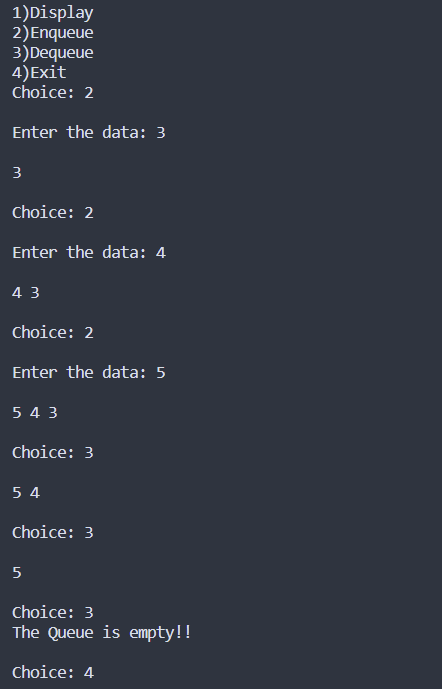
\includegraphics[]{Cycle_2/Outputs/Queue.png}

\section{Result}
The queue operations using linked list were performed successfully. Output was verified.
